\chapter{研究背景}
\label{chap:haikei}

本章では手書きメモ・イラストを扱う既存のシステムの現状と、その問題点を整理する。

\newpage

\section{手書きのメモ・イラスト}
手書きによってメモやイラストを表現するのは、鉛筆等の筆記具と紙さえあればすぐに記録でき、また美麗な作品を描くことを目的としなければ、
特別な技量も要求されないため、情報を記録・表現する手法として広く普及している。
計算機の登場によりテキスト編集支援機能が充実したため、文章のみで完結する内容であれば手書きではなくタイピングによって記録するように置き換わったが、
アイデアのような文章のみでは表現しづらい構造を持った概念を表現する場合は文字と図を自在に混合させて配置できる手書きメモの方が適している。
また、テキストによってメモをとる場合はキーボードのような専用のハードウェアや、それらを使いこなすタッチタイピング等の技量が必要であるという問題点があるが、
手書きの場合は紙やペン等の筆記具が扱えれば良いため、ハードウェアや技能を必要とするテキスト入力と比較してより多くの人々が利用できる手段であると言える。

\section{タッチ・ペンインターフェースの普及}

\begin{figure}[htbp] \begin{minipage}{0.5\hsize}
                         \begin{center} {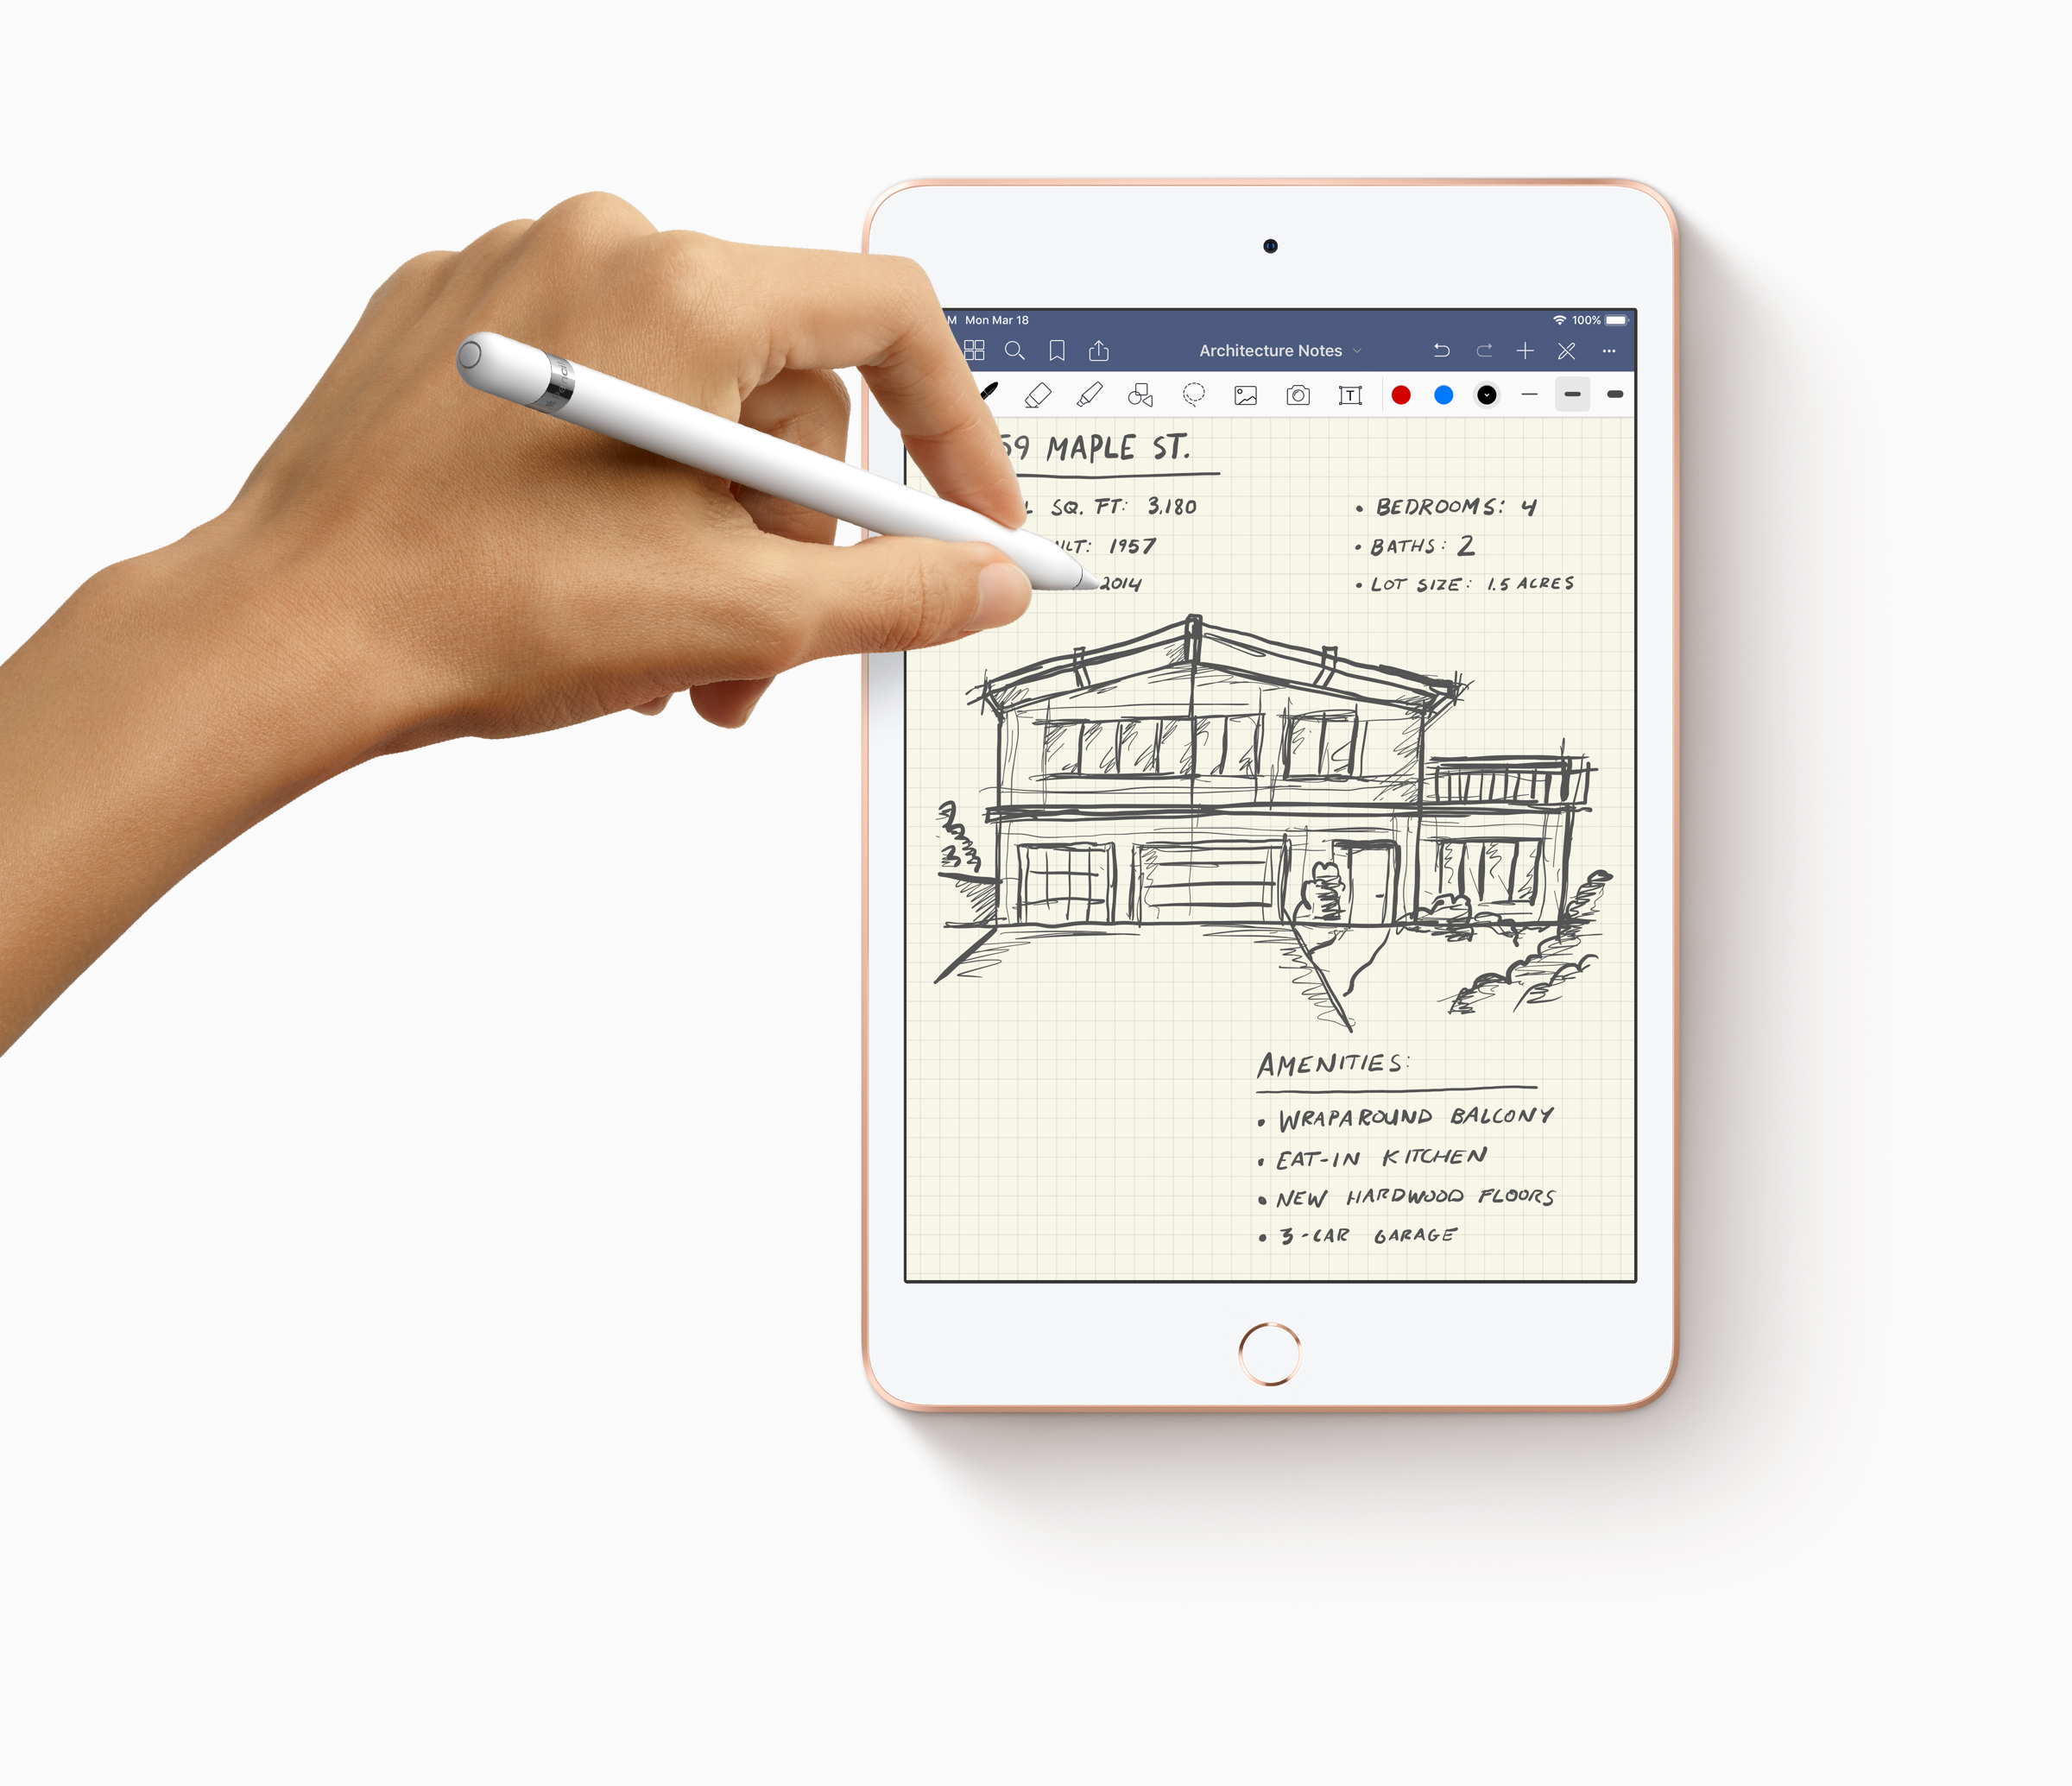
\includegraphics[width=40mm]{images/ipadmini.jpg}}
                         \end{center} \caption{iPad}
\end{minipage} \begin{minipage}{0.5\hsize}
                   \begin{center} {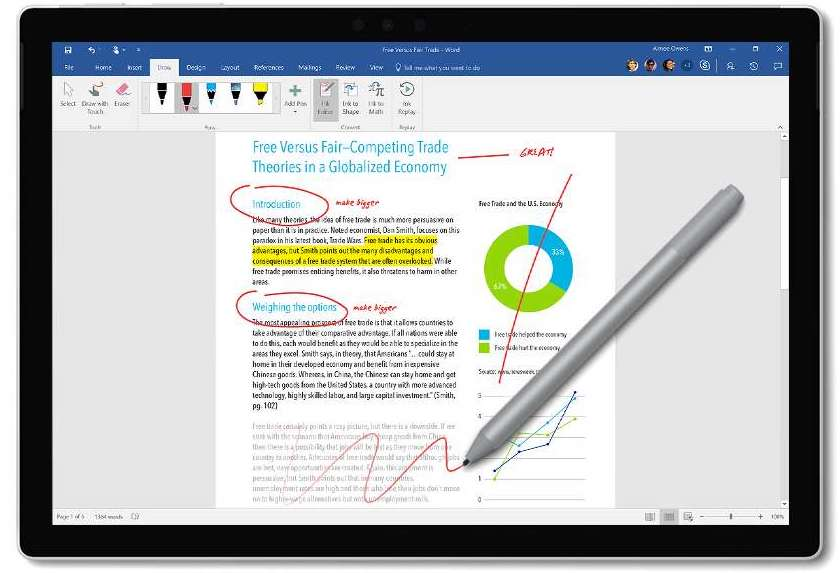
\includegraphics[width=40mm]{images/surface.jpg}}
                   \end{center} \caption{Surface}
\end{minipage}
\end{figure}

かつてはノートやスケッチブック等の紙の上で記録されていた手書きメモだが、タッチパネルやスタイラスペン等のインターフェースを備えたデバイスの普及に伴い、
計算機上で手書きメモを取ることが一般化してきた。
手書きメモやイラストを計算機の上で描く場合、マウスやトラックパッド等のポインティングデバイスではなく、
ペンインターフェースが好ましいとされるが、iOS\footnote{https://www.apple.com/jp/ios/}やWindows\footnote{https://www.microsoft.com/ja-jp/windows}、
ChromeOS\footnote{https://www.google.com/chromebook/}等の主要なプラットフォームで
スタイラスペンを備えた機種が充実しているため手書きでメモやイラストを描く環境は充分に整っている。

\section{計算機上の手書きメモ・イラスト}
計算機上でメモやイラストを作成する場合、以下のような編集支援機能を利用することができる。
\begin{itemize}
    \item コピーやペースト
    \item UndoやRedo
    \item オブジェクトの移動や変形
    \item 複数のレイヤーの合成
\end{itemize}
これらの機能は紙という物理的なメディアの上では実現不可能であったが、計算機の進化によって大抵のアプリケーションに搭載されるようになったため、
より便利に手書きのメモやイラストを作成することができるようになった。

\section{手書きデータを表現する画像ファイルフォーマット}
手書きのメモを作成する段階では計算機による便利な編集支援機能を利用できるようになったが、それを保存するファイルのフォーマットの機能は大きく制限されている。
一般的に出力先としてJPEGやPNG等のビットマップ画像が用いられているが、この種のフォーマットはレイヤーや編集履歴等の構造は保持されず、
描いたもの全てがピクセルの集合として統合・変換されるほか、一部のメタデータを除いて基本的にピクセル以外の情報を保存することができないため、紙と比較して本質的に進歩していない。
そのため画像ファイルを参照するには保存するディレクトリを予め取り決めたり、タイムスタンプを頼りに時系列順でソートしたりと、紙の上で記録していたときの不便さをそのまま引き継いでしまっている。

\section{手書きデータを扱う既存のシステム}

\subsection{デジタルペン}

\subsubsection{Anoto}

\begin{figure}[htbp] \begin{minipage}{0.5\hsize}
                         \begin{center} \fbox{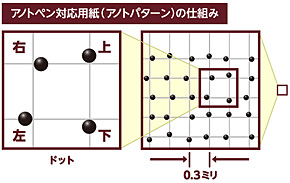
\includegraphics[width=50mm]{images/anoto1.jpg}}
                         \end{center} \caption{Anotoパターン} \label{fig:anoto1}
\end{minipage} \begin{minipage}{0.5\hsize}
                   \begin{center} \fbox{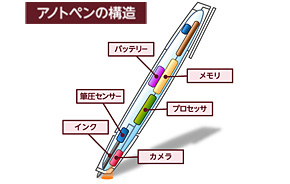
\includegraphics[width=50mm]{images/anoto2.jpg}}
                   \end{center} \caption{専用のペン} \label{fig:anoto2}
\end{minipage}
\end{figure}

Anotoによるデジタルペンは、Anotoパターンと呼ばれる微細なドットが印刷された専用の用紙に、カメラを内蔵したペンで記入することにより手書き入力をデータ化するシステムである。
専用の紙とペン以外に特殊なタブレット機器や読み取り装置を必要としないが、あくまで物理的な紙の上に記入しているためUndoやRedo等の計算機による編集支援機能は利用できない。

\subsection{メモアプリケーション}
手書きデータを効率よくメモとして扱えるようにしたシステムを解説する。

\subsubsection{iOSのメモ}

\begin{figure}[htbp]
    \begin{center}
        {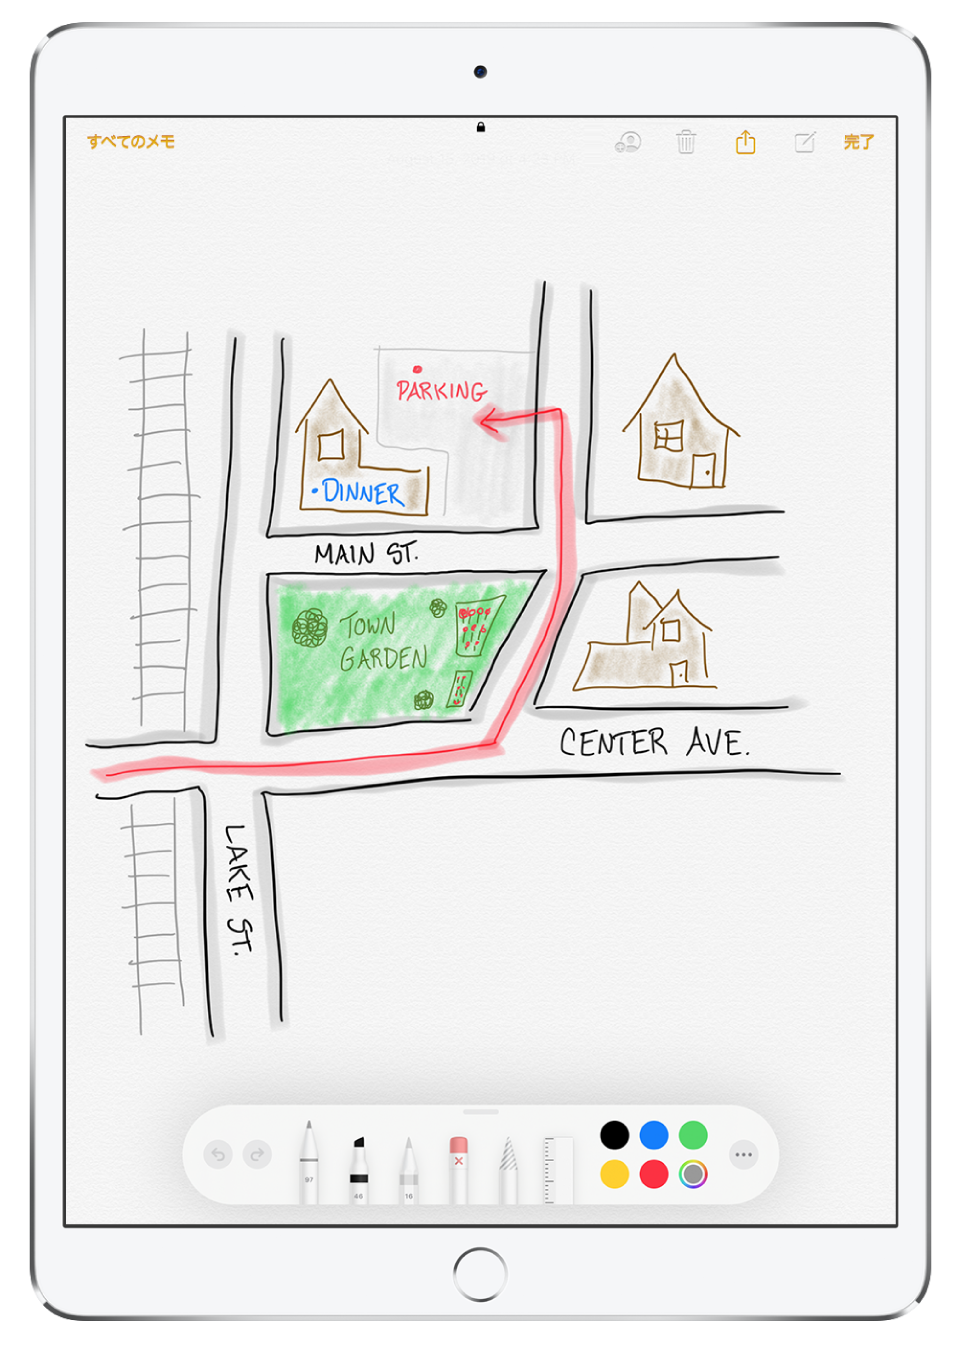
\includegraphics[width=50mm]{images/applememo.png}} \end{center}
    \caption{iOSのメモ}
\end{figure}

AppleのiPadにはメモアプリケーションが標準でインストールされており、指やApple Pencilを用いて素早く手書きメモを取ることを可能で、
さらにUndoやRedo等の編集支援機能を備えている。一方で描いた手書きメモは画像として保存されるのみで、
後から検索する手立てがなく、ファイル名の規則を決めたり保存先フォルダを分ける等の工夫が運用上必要とされる。

\subsubsection{Evernote}

\begin{figure}[htbp]
    \begin{center}
    {
\includegraphics[width=50mm]{images/testimage.png}} \end{center}
    \caption{Evernote}
\end{figure}

Evernote Corporationが開発するEvernoteは指やスタイラスペンで手書きのメモやスケッチを記録することができる。
手書きの文字を認識することで後からテキストによって検索する機能を備えているが、これは手書きメモをテキストに変換することで実現しているため、
図形や描いたものの形状等のグラフィカルなデータから手書きメモを参照することはできない。

\subsubsection{Google Keep}

\begin{figure}[htbp]
    \begin{center}
    {
\includegraphics[width=50mm]{images/testimage.png}} \end{center}
    \caption{GoogleKeep}
\end{figure}


Googleが開発するGoogle Keepも、Evernoteと同様にテキストによって検索することも可能である。
さらに画像や手書きメモ内にある文字を認識してテキストとして抽出する機能があるが、やはりこれも手書きメモ内の文字を
テキストに変換するというアプローチであるため、Evernoteと同様の問題を抱えている。

\subsection{イラスト投稿・共有システム}
Web上で手書きのイラストを投稿・共有可能にするシステムを解説する。
これらのシステムは基本的に完成されたアート作品を投稿するのが主な用途であり、メモを素早く記録する手段
として使われることはないが、様々な工夫によってイラストの参照や管理の問題の改善に取り組んでいる。

\subsubsection{Pixiv}

pixiv Inc.が開発するPixivでは、投稿したイラストに複数のタグを付加することができる。
また共通のタグを持つ他のイラストを関連イラストとして下部に表示する機能を備えているため、作者を横断して共通するテーマの他のイラストを参照することができる。

\begin{figure}[htbp]
    \begin{center}
    {
\includegraphics[width=50mm]{images/testimage.png}} \end{center}
    \caption{Pixiv}
\end{figure}


\subsubsection{ニコニ・コモンズ}

ドワンゴが開発するニコニコ動画の関連サービスであるニコニ・コモンズでは、イラストも含めた素材の親子関係を記述するコンテンツツリーという機能が実装されている。
これによりある作品の元になった作品や、ある作品を元にした他の作品を参照することができる。
ただし登録は子作品の投稿者が手動で行わなければならないという制約があるため、全ての作品のコンテンツツリーが漏れなく記述されているわけではない。

\begin{figure}[htbp]
    \begin{center}
    {
\includegraphics[width=50mm]{images/testimage.png}} \end{center}
    \caption{ニコニ・コモンズ}
\end{figure}


\section{テキストの進化}
手書きのメモやイラストと同様に紙の上で表現されていたテキストは計算機の登場により以下のような機能を獲得した。
\begin{itemize}
    \item ハイパーリンク\\
    ハイパーテキストでは文章間リンクを示すハイパーリンク機能が利用でき、関連情報への素早いアクセスが可能になった。
    \item Web\\
    インターネット技術の進化とWebの普及によって、世界中に存在する様々なドキュメントへ瞬時にアクセスすることが可能になった。
    \item 共同編集\\
    Wikiのようなコラボレーションツールによって、場所や人数に制約を受けない共同編集が可能になった。
\end{itemize}
これにより参照・管理・再利用が難しいという問題点を解決するに至った。

\section{手書きデータを扱う既存システムの問題点}
手書きデータを扱うシステムは数多く存在し活用されているものの、画像ファイルのフォーマットの機能が制限されているため、
計算機の進化によって得られる便利な機能を享受できていない。また、

\section{まとめ}
手書きメモ・イラストは広く浸透した情報の記録手法であるものの、紙というフォーマットの制約によって使い勝手が制限されている。
一方でデジタル化された手書きメモ・イラストの作成や閲覧を支援するシステムが広く利用されているが、
これらは計算機上で手書きの利用形態を再現したに過ぎず、本質的な問題は解決されていない。
次章では上記のような問題点を解決し、これまでの手書きメモ・イラストの在り方にとらわれない次世代のフォーマット「ハイパーイラスト」と、
それらを容易に管理・再利用できるシステム「手書きベースWiki」を提案する。